\section{Résolution d'équation différentielles}

Cette première partie traite de l'implémentation des méthodes numériques de résolution
d'équation différentielle.\\
Dans un premier temps, nous avons défini une répresentation des problèmes de Cauchy.\\
La solution initiale $y0$ est représentée par un array de float. La fonction différentielle est décrite
par une fonction Python $f(t, y)$ qui retourne un array de la même taille que $y$.

\subsection{Implémentation générique}

Nous avons implémenté quatre méthodes : Euler, Heun, point milieu et Runge Kutta.\\
Pour chaque méthode, on retrouve une fonction \texttt{step\_<name>(y, t, h, f)} qui effectue un seul pas de la méthode et 
une fonction \texttt{meth\_n\_step(y0, t0, N, h, f, step\_method)} qui applique la méthode sur N pas de taille constante.
Enfin, la fonction \texttt{meth\_epsilon(y0, t0, tf, eps, f, step\_method)} affine le pas jusqu’à atteindre une précision donnée.\\
Cette implémentation générique évite la duplication de code et facilite l'ajout d'une nouvelle méthode.


\subsection{Applications sur des équations différentielles connues}

Pour les quatres méthodes, la solution obtenue et la solution exacte sont extrêment proches pour la dimension 
une. Le tracé des résultats obtenus sont similaires pour les méthodes de Heun, du point milieu et de Runge
Kutta pour les dimensions une et deux. La figure~\ref{fig:heun} montre les résultats obtenus par la méthode de Heun.

\begin{figure}[ht]
    \centering
    \begin{subfigure}[b]{0.24\textwidth}
        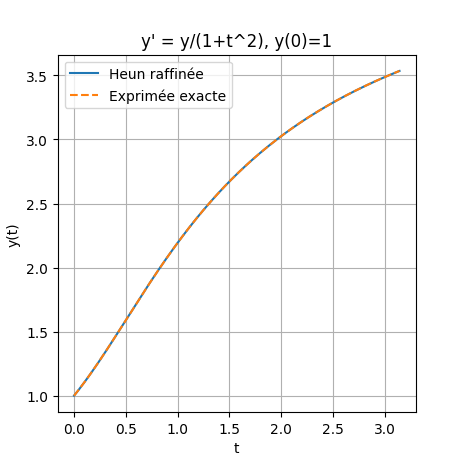
\includegraphics[width=\linewidth]{img/heun1.png}
    \end{subfigure}
    \hspace{0.01em}
    \begin{subfigure}[b]{0.49\textwidth}
        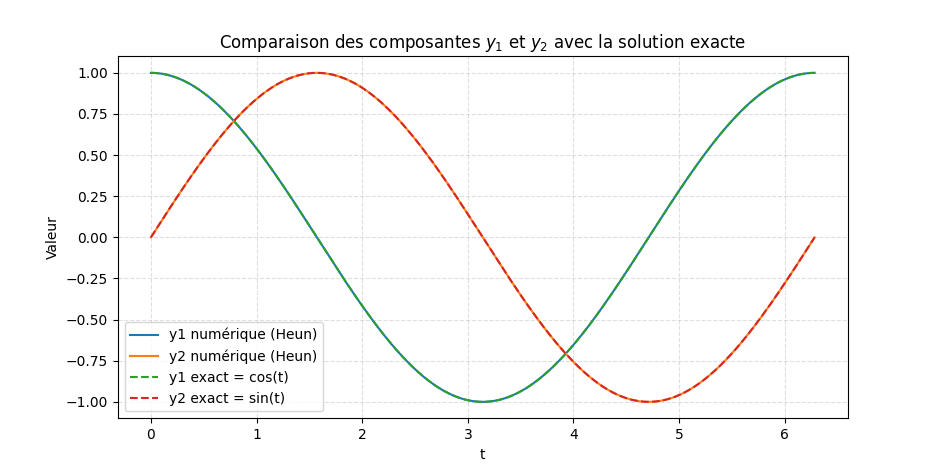
\includegraphics[width=\linewidth]{img/heun2.png}
    \end{subfigure}
    \hspace{0.01em}
        \begin{subfigure}[b]{0.24\textwidth}
        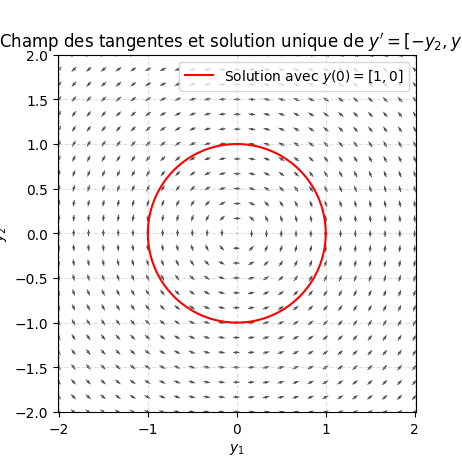
\includegraphics[width=\linewidth]{img/heun3.png}
    \end{subfigure}
    \caption{Résultats de la méthode de Heun}
    \label{fig:heun}
\end{figure}

Cependant, nous observons que la méthode d'Euler est moins précise
que les autres méthodes pour la dimension deux, comme le montre la figure~\ref{fig:euler}.

\begin{figure}[ht]
    \centering
    \begin{subfigure}[b]{0.24\textwidth}
        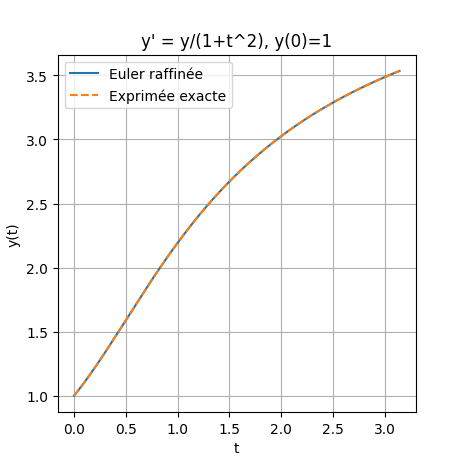
\includegraphics[width=\linewidth]{img/euler1.png}
    \end{subfigure}
    \hspace{0.01em}
    \begin{subfigure}[b]{0.49\textwidth}
        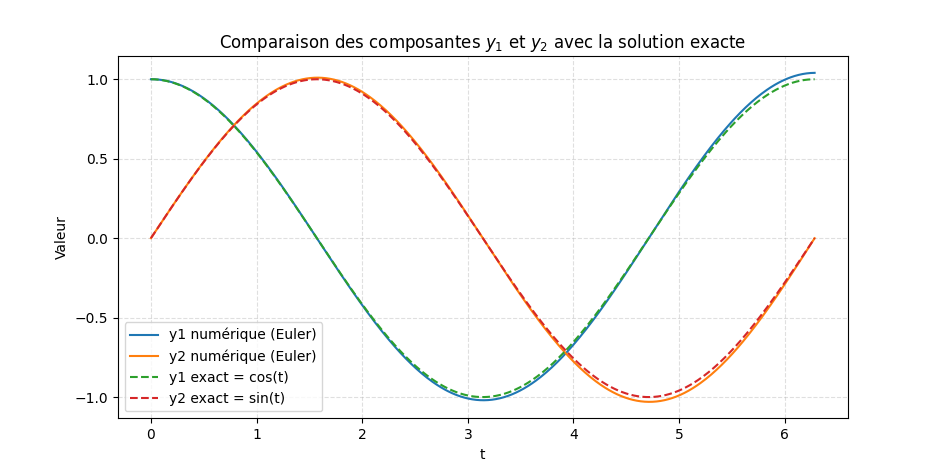
\includegraphics[width=\linewidth]{img/euler2.png}
    \end{subfigure}
    \hspace{0.01em}
        \begin{subfigure}[b]{0.24\textwidth}
        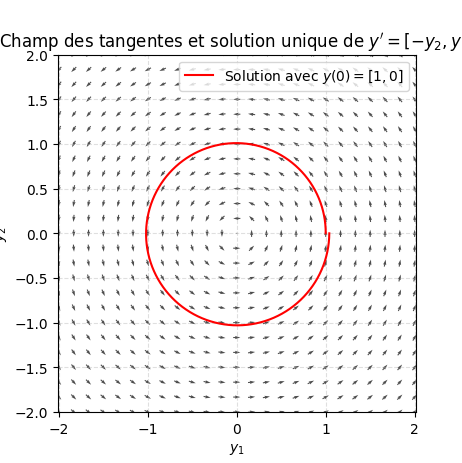
\includegraphics[width=\linewidth]{img/euler3.png}
    \end{subfigure}
    \caption{Résultats de la méthode d'Euler}
    \label{fig:euler}
\end{figure}

Les erreurs rencontrées sont en majorité des erreurs d'arrondis. En effet, l'approximation de la solution exacte par la 
méthode numérique introduit une erreur à chaque pas. De plus, pour des pas trop grand, la solution peut diverger.